\documentclass[a4paper, 12pt]{report}
\usepackage{amsmath}
\usepackage{amssymb}
\usepackage{graphicx}

\newcommand{\url}[1]{\textit{#1}}
\newcommand{\bt}[1]{\textbf{#1}}
\newcommand{\ubt}[1]{\textbf{\underline{#1}}}
\newcommand{\sps}{\\[0.2cm]}
\newcommand{\spn}[1]{\\[#1cm]}
\newcommand{\refn}[1]{\textbf{(\ref{#1})}}
\newcommand{\NI}{\noindent}
\newcommand{\beq}{\NI$\displaystyle}
\newcommand{\eeq}{$}
\newcommand{\eeqn}{$\\[0.3cm]}
\newcommand{\dsp}{\displaystyle}

\renewcommand*\contentsname{Table of Contents}
\renewcommand{\baselinestretch}{1.5}

\linespread{1.5}
\setlength\parindent{0pt}
\newcommand\Laplace{\mathlarger{\mathlarger{\mathscr}}}
\begin{document}

\begin{titlepage}
\begin{center}
\textbf{\large {BASIC FLUID EQUATIONS IN DIFFERENT COORDINATE SYSTEMS}}
\\[35pt]
BY
\\[20pt]
\textbf{HASSAN, ABDULRAZAQ TIJANI }
\\[20pt]
MATRIC NUMBER: 16/56EB075

\vspace{2cm}
A PROJECT SUBMITTED TO THE DEPARTMENT OF MATHEMATICS, FACULTY OF PHYSICAL SCIENCES, UNIVERSITY OF ILORIN, ILORIN, NIGERIA, IN PARTIAL FULFILLMENT OF THE REQUIREMENTS FOR THE AWARD OF BACHELOR OF SCIENCE DEGREE (B. Sc.) IN MATHEMATICS.
\\[35pt]
JUNE 2021.
\end{center}
\end{titlepage}

\pagenumbering{roman}
\newpage
\begin{center}\section*{CERTIFICATION}\end{center}
This is to certify that this project work was carried out by \textbf{Hassan Abdulrazaq Tijani} with matriculation number \textbf{16/56EB075} and approved as meeting the requirement for the award of the Bachelor of Science (B. Sc.) degree of the Department of Mathematics, Faculty of Physical Sciences, University of Ilorin, Ilorin, Nigeria.

\vspace{.99in}
\noindent
\dotfill			\hfill			\dotfill\\
\textbf{Dr. E. O. Titiloye} ~~~~~~~~~~~~~~~~~~~~~~~~~~~~~~~~~~~~~~~~~ 
Date\\
Supervisor

\vspace{.99in}
\noindent
\dotfill			\hfill			\dotfill\\
\textbf{Prof. K. Rauf} ~~~~~~~~~~~~~~~~~~~~~~~~~~~~~~~~~~~~~~~~~~~~~~ Date\\
Head of Department

\vspace{.99in}
\noindent
\dotfill			\hfill			\dotfill\\
\textbf{Prof . T. Oluyo} ~~~~~~~~~~~~~~~~~~~~~~~~~~~~~~~~~~~~~~~~~~~~~ Date\\
External Examiner
\newpage
\begin{center}\section*{DEDICATION}
This project is dedicated to God,my beloved parents and Africa's underprivileged children.%you may decide to change this anytime
\end{center}

\newpage
\begin{center}
\section*{Acknowledgement}
\end{center}
All praises glorifications are for the almighty Allah, my creator and sustainer
of the world, whom I owe every deep sense of gratitude over the
years for sparing my life from the beginning to the end of my course in
the prestigious University of Ilorin.
My profound gratitude to Dr. E. O. Titiloye who has been the ideal project supervisor , for his advice, and patient encouragement
aided the writing of the project in innumerable ways. I pray
almighty God bless him.
I express my thanks to  Prof. K. A Rauf who is the Head of Department
(H.O.D) for being a true father, creating accomodating environment for we students to excel in our studies. My sincere gratitute to my level adviser,Dr. Idayat. F. Usamot , for her fatherly advice on our academics, may Allah be with her and her family.
I also appreciate the immeasuraable effort of my lecturers in the department including Prof. J. A Gbadeyan, Prof. O. T Opoola, Prof. O. M.
Bamigbola, Prof M. O Ibrahim, Prof. O. A. Taiwo,Prof R. B. Adeniyi, Prof A. S. Idowu, Prof. M. S. Dada, Prof. K. O. Babalola, Dr. Olubunmi. A. Fadipe-Joseph,Dr. Yidiat. O. Aderinto, Dr. Catherine. N. Ejieji, Dr.B. M. Yisa, Dr J. U. Abubakar, Dr. K. A. Bello, Dr. Gata. N. Bakare, Dr T. O. Olotu, Dr. B.M. Ahmad, Dr O. A.Uwaheren, Mr Odetunde and all other members of staff of the department of mathematics, who contributed greatly to my academic excellence, obtained during my period of study in the department. May God bless them all.\newline
I am highly indebted to my loving and respectable family; my gold, my
parents Mr Hassan Tijani and Mrs Hawau Tijani , thank you for birthing me, raising me and teaching me the essential lessons of life and i am forever grateful; my siblings Lukman hassan and biliki hassan may almighty Allah be with you and bless you all in all abundantly ramifications.\newline
Also to my special friends,Adeola Joseph, Azeez ibrahim, Austin ebiale (OPAY), Odion,Fatiu Abdulrazaq (Al-taggana bil quran),Timileyin David, Muyiwa reuben , Hassan and Hussien suliamon, Alade Khalid and so on  for their undying support, advice and assistance to my dedication.\newline
I will love to give a special shout-out to the greatest afrobeat artist/singer Wizkid Ayo Balogun whose music has been an inspiration throughout my life and i thank you for the special album Made in Lagos which changed my life and God bless the entire wizkid F.C. for their Love and cooperation towards this movement.\newline
Special thanks to the the entire student of mathematics department for their cooperation and assistance towards my work.




\newpage
\begin{center}
\section*{Abstract}
\end{center}
This project studies the flow of fluids in three dimensional coordinate considering the continuity equation and Navier-strokes equation in Cartesian coordinate and moreover converting to spherical coordinate , these equations are not autonomous but subject to the Newtons law of motion




\newpage
\pagenumbering{arabic}
\tableofcontents

\chapter{General Introduction}
\section{Background of Study}

Fluid mechanics is the branch of science concerned with the mechanics of fluids (liquids, gases, and plasmas) and the forces acting on them. It deals with the study of all fluids. It has applications in a wide range of disciplines, including mechanical, civil, chemical and biomedical engineering, geophysics, astrophysics, and biology. 
It can be divided into fluid statics, the study of fluids at rest, and fluid dynamics, and the study of the effects of fluid motion. 
The study of fluid mechanics goes back at least to the days of ancient Greece , when Archimedes investigated fluid statics and buoyancy and formulated his famous law known now as the Archimedes’ principle, which was published in his work ”On Floating Bodies” generally considered to be the first major work on fluid mechanics.
Fluid mechanics is also a branch of continuous mechanics which deals with the relationship between forces, motion and statical conditions in continuous materials. This study areas deals with many problems such as surface tensions , fluid statics , flow on enclosed bodies or round bodies(solid or otherwise ) flow stability etc.


\newpage
\section{Scope of Study}
This project work is subject to the law of motion even as fluid flow leads to the equation of motion. It also focuses on flow in spherical coordinate and its conversion from cartesian coordinate to sphrical coordinate.


\newpage
\section{Aim and Objectives}
The aims of this research is to study the flow of fluids through different coordinate system and the conversion from cartesian to spherical coordinate.\\



\newpage
\section{Definition of Relevant Terms}
\subsection{Fluids}
A fluid is any substance that flows or a substance that deforms continuously when subjected to an external shearing stress. This term is used for both liquids and gases.
One can easily define Fluids in the manner of how they respond, i.e. deforms or flow when they are subjected to a force in a specific situation such as shear stress Edward N. (2007).



\subsection{Fluid Mechanics }
Fluid mechanics is the study of the behaviour of fluids under the influence of force.
It is divided into two broad’s topic namely:
(i)	Fluid static.
(ii)Fluid Dynamics.


\subsection{Fluid Statics}
It is the study of Fluids at rest. It can also be define as the forces that holds fluids in static equilibrium. It is based on Newton’s first law of motion. .i.e. there are no shear
Stress present (a shear results from a velocity gradient).
.

\subsection{Fluids Dynamics}
This is the study of fluids in motion and the forces that keeps them in motion.

\subsection{Deformation}
This is the change in shape of mass of fluid when a force is been applied on it . The shear stress exists during the deformation).

\subsection{Continuous Deformation}
This occurs when a fluid continues to deform for as long as the force is applied on it.
\subsection{Types of Fluids}
(1).	 Ideal Fluid
A  Fluid which is incompressible and have no viscosity and surface tension is known as an Ideal fluid. Ideal fluid is only an imaginary fluid, such fluids do not really exists.


(2). 	Real Fluid
A fluid which possesses viscosity, surface tension, compressibility and density is known as real fluid. All the fluids in actual practice are real fluids and are actually available in nature.




(3). Newtonian Fluid

A real fluid in which the shear stress is directly proportional to the rate of shear strain (or velocity gradient), is known as Newtonian fluid.

(4). Non-Newtonian Fluid
A real fluid in which the shear stress is not proportional to the rate of shear strain (or velocity gradient) is known as non-newtonian fluid.


(5).  Uniform Fluids 
Fluids are said to be uniform if its properties are the same at all points .Fluids are not uniform excepts when temperature and pressure are the same throughout.


(6).  Ideal Plastic Fluid
A fluid in which shear stress is more than the yield value and shear stress is proportional to the rate of shear strain (or velocity gradient) is known as ideal plastic fluid.



(7).  Invisid Fluid

An invisid fluid (Non-viscous) is a type of fluid even when in motion is incapable of sustaining a shear stress. In reality no fluid is non-viscous, however the effects of viscosity is negligible or very small such as water and air.


\subsection{Properties Of Fluids}
(1).	Viscosity:
 This is the fluid property which measures the resistance to flow. It is a quantitative measure of fluid resistance to flow. For example different fluid have different viscosity. i.e. the viscosity of mercury is higher than water while that of water is higher than air. It is denoted as $\mu$ .

(2).	Surface Tension:
 This is one of the important fluid property. It is well observed that some insects could walk on water without their body getting wet while some can’t. It is thereby defined as the force per unit length acting in the surface of the right angle to one side of a line drawn in the surface.
 
 
(3).Density: Density is defined as the ratio between mass and volume.. It is denoted as . The s.i unit is .


(4).	Relative Density: It is defined as the ration of mass density of substance to some standard mass density. It is unit less.


(5).	Specific Weight: This is defined as the weight per unit volume, which varies from one point to point dependent on the varational of gravity(g) .

\subsection{Fluid Flow}
This is defined as the movement of real fluids.

\subsection{Types of Fluid Flow}
(1).	Steady and Unsteady Flows:
Steady flow is defined as that type of flow in which the fluid characteristics like velocity, pressure, density, etc. at a point do not change with time.

 Unsteady flow is that type of flow in which the velocity, pressure or density at a point changes with respect to time.
 
(2).	Compressible and Incompressible Flows:
Compressible flow is that type of flow in which the density of the fluid changes from point to point or in other words the density ($\rho$) is not constant for the fluid.

Incompressible flow is that type of flow in which the density is constant for the fluid flow. Liquids are generally incompressible while gases are compressible.


(3).Uniform and Non-uniform Flows:
Uniform flow is defined as that type of flow in which the velocity at any given time does not change with respect to space (i.e length of direction of the  flow).

Non-uniform flow is that type of flow in which the velocity at any
given time changes with respect to space.


(4).Rotational and Irrotational Flows:
Rotational flow is that type of flow in which the fluid particles while owing along streamlines also rotate about their own axis. And if the fluid particles while owing along streamlines, do not rotate about their
own axis then that type of flow is called irrotational flow.

(5). 	Laminar and Turbulent Flow:
Laminar flow is defined as that type of flow in which the fluid particles
move along well-defined paths or streamline and all the streamlines
are straight and parallel. Thus the particles move in laminas or layers
gliding smoothly over the adjacent layer. This type of flow is called
streamline flow or viscous flow.
Turbulent flow is that type of flow in which the fluid particles move in
zig-zag way. Due to the movement of fluid particles in a zig-zag way, the eddies formation takes place which are responsible for high energy loss.
For a pipe flow, the type of flow is determined by a non-dimensional
number VD/v called the Reynolds number.
Where
D = Diameter of pipe.

V = Mean velocity.

v = Kinematic viscosity of fluid.


If the Reynold number is less than 2000, the flow is called laminar.


If the Reynold number is more than 4000, it is called turbulent flow.


If the Reynold number lies between 2000 and 4000, the flow may be laminar or turbulent.
.
.\subsection{Types of Flowlines}

(1). PATHLINE
A pathline is a path followed by a 
fluid particle in motion. A pathline
shows the direction of particular particle as it moves ahead. In general,
this is the curve in 3-dimensional space. However, if the conditions are
such that the 
ow is 2-dimensional, the curve becomes 2-dimensional..

(2). STREAKLINE
The streakline is a curve which gives an instantaneous picture of the
location of the fluid particles which have passed through a given point.

Examples.

(a) In an experimental work to trace the motion of fluid particles,
a coloured dye may be injected into the following 
fluid and the
resulting coloured lament lines at a given location given by the
streaklines.

(3). STREAMLINE
A streamline can be defined as an imaginary line within the flow so
that the tangent at any point on it indicates the velocity at that point.
Equation of a streamline in a 3-dimensional flow is given as;..


 $\displaystyle  \frac{\partial x}{u} =  \frac{\partial y}{v}= \frac{\partial z}{w}$\\.

EXAMPLE
(a) For a 3-dimensional flow, the velocity distribution is given by u =
-x; v = 3-y; w = 3-z. What is the equation of a streamline
passing through (1; 2; 2)?.
.

Solution
Given: u =-x, v = 3-y, w = 3-z
Equation of a streamline passing through (1; 2; 3):
The streamlines are defined by,

.
 $\displaystyle  \frac{dx}{u} =  \frac{dy}{v} =\frac{ dz}{w}$\\.

Substituting for u, v and w, we get

$\displaystyle  \frac{dx}{-x} = \frac{\ dy}{3-y} =\frac{\ dz}{3-z}$\\

Considering the expressions (i) and (ii) and integrating, we get
\begin{equation}
	\int  \frac{\ dx}{-x} =  \int \frac{\ dy}{3-y} \\
\end{equation}
	-$\log_e x = -\log_e (3-y) + c_1$
	(where C1 = constant of integration)	
Since the streamline passes through $x=1, y=2, C_1 =0$.\\
$(x)^-1 = (3-y)^-1  or x = (3 - y)$
.
.\\
Considering the expressions (i) and (iii), and integrating, we get,\\

\begin{equation}
	\int  \frac{\ dx}{-x} =  \int \frac{\ dz}{3-z} \\	
\end{equation}.
	-$\log_e x = -\log_e (3-y) + c_2$

(where $C_2$ = constant of integration)
Since the streamline passes through $x=1, y=2, C_2 =0$.\\
$(x)^-1 = (3-z)^-1  or x = (3 - z)$
\\
The streamline equation is :
$x = (3-y) = (3 -z)$



  

\subsection{What Is Heat Transfer}
Heat transfer is a discipline of thermal engineering that concerns the generation, uses and exchange of thermal energy between physical system. Heat transfer is classified into various mechanics such as thermal convention, thermal conduction, thermal radiation and transfer of energy by phases changes.


Heat transfer describe the flow of heat (thermal energy) due to temperature difference and the subsequent temperature differences and the subsequent temperature distribution and changes.


\subsection{Types of Heat Transfers}
(1).Conduction: It is the heat transfer through stationary matter by physical contact. E.g. Heat Transferred between the electric burner of a stove and the bottom of a pot is transferred by conduction

(2).Convention: It is the heat transfer by the macroscopic movement of fluid. This is the type of transfer that takes place in a forced air furnace and in weather systems.

(3).Radiation: Heat transfer by radiation occurs when micro-waves, infrared radiation, visible light or another form of electromagnetic radiation is emitted or absorbed. E.g warming of the earth by the sun.

\section{Equations Of Motion}
In Fluids mechanic , Equations of motion is a great subtpoic under fluid and it includes  the continuity Equation,the Navier-stokes equation and conservation of thermal energy  which yields the energy equation.
\subsection{Continuity Equation}
This continuity equation states that in case of a steady flow, the amount of fluids flowing past one point must be the same flowing past another points, or mass flow rate is constant. 
It is essentially a statement of the law of conversation of mass. 
The explicit formula of the continuity equation is
		$A_1V_1$ = $A_2V_2$.\newline
		consider a pipe  having two Points A and B:
		
		Let $A_1$ = Area of the pipe at point A\newline
		$V_1$ = Velocity of the pipe flowing through A\newline
		$\rho_1$ = Density of the fluidat point A \newline
		
		Let $A_2$ = Area of the pipe at point B \newline
		$V_2$ = Velocity of the pipe flowing through B\newline
		$\rho_2$ = Density of the fluid at point B \newline
		
		$\rho_1$ $A_1$ $V_1$ = The total quantity of fluid passing through point A \newline
		$\rho_1$ $A_2V_2$ = and the total quantity of fluid passing through point B \newline
		\begin{center}
			From the theorem of continuity, we deduce that:
		\end{center}
		\begin{center}
			
			\begin{equation}
				\rho_1 A_1 V_1 = \rho_1 A_2V_2 
			\end{equation}
			
		\end{center}
		Equation (1.3) is applicable to the compressible as well as incompressible fluids. It is called Continuity Equation. In case of incompressible fluids,since there is not occurrence of change in density of fluid, that is, $\rho_1$ = $\rho_2$
		,the continuity equation reduces to:
		\begin{center}
			$A_1$ $V_1$= $A_2V_2$
		\end{center}
This proves that for an incompressible fluid is undergoing steady flow , the product of cross sectional area and the speed must be the same for any two random point and this is called the equation of continuity.

\subsection{Navier stokes}

The Navier stokes Equation is a fundamental differential equation that describe the flow of an incompressible fluids.
 \begin{equation}
 	\frac{\partial \rho}{\partial t} + \overrightarrow{\nabla} \cdot(\rho \overrightarrow{u}) =o
 \end{equation}
\begin{equation}
	\frac{\partial(\rho \overrightarrow{u})}{\partial t} + \overrightarrow{\nabla} \cdot[\rho\overline{\overline{u\otimes u}}] = -\overrightarrow{\nabla p} + \overrightarrow{\nabla} \cdot\overline{\overline{\tau}} + \rho\overrightarrow{f}
\end{equation}.
\begin{equation}
	\frac{\partial}{\rho e}{\partial t} + \overrightarrow{\nabla} \cdot ((\rho e + p)\overrightarrow{u}) = \overrightarrow{\nabla} \cdot (\overline{\overline{\tau}}\cdot \overrightarrow{u}) + \rho\overrightarrow{f} \overrightarrow{u} + \overrightarrow{\nabla}\cdot(\overrightarrow{\dot{q}}) + r
\end{equation}
\subsection{Energy Equation}

Energy is the quantitative property that must be transferred to an object in order to perform work on, or to heat, the object. Energy is a conserved quantity, the law of conservation of energy state that energy can be converted in form, but not created or destroyed. The SI unit of energy is the joule, which is the energy transferred to an object by the work of moving it a distance of 1 metre against a force of 1 newton Smith, Crosbie (1998).\\

In fluid mechanics one of the basic equations is energy equation. The
different types of energy  of flowing liquids considered in fluid are as follows:Potential energy: In relational concept with
the generally known form of potential energy, it is due to configuration
or position above some suitable datum (or elevation) line. It is usually
denoted by z.\newline
Velocity head or kinetic energy: This is due to velocity of flow liquid and is measured as $\frac{V^2}{2g}$  where, V is the velocity of flowing \newline and g is the acceleration due to gravity (g = 9.81) .\newline
pressure energy: This is due to the pressure of liquid and reckoned as
$\frac{p}{w}$where, p is the pressure, and w is the weight density of the liquid.\newline
Total head/energy:
Total head of a liquid particle in motion is the sum of its potential head,kinetic head and pressure head. Mathematically\newline
\begin{center}
	Total Head(H) =z + $\frac{V^2}{2g}$ + $\frac{p}{w}$ m of a liquid.
\end{center}



\pagebreak
\chapter{Literature Review}
\section{Introduction}
Fluid mechanics is a wide ranged field that revolves around laws of applied mechanics and results from involving the physical laws of momentum Conservation of mass and energy. where the conservation of mass yields the Navier-stokes equation and conservation of thermal energy yields the energy equation.

 All these equation are known as equation of motion .Moreover through these equations of motion flow of fluids through a particular co-ordinate can be converted to another coordinate. (spherical, Cartesian and cylindrical). Which will be treated further in the course of this project work.

\section{Coordinate System}
A coordinate system is a rule for mapping pairs of numbers to points in a plane.\newline
In geometry, a coordinate system is a system that uses one or more numbers or coordinate to uniquely determine the position of the points or other geometric element on a manifold such as Euclidean space.
A coordinate system is not just a set of axis, it is a set of rules for mapping a pair of numbers onto a points in plane Eric W.(1999).


Different coordinate system correspond to different rules. The polar coordinate has rules that are different than the rules of the XY coordinate system. Other coordinate system yet have another rules.
The use of a coordinate system allows problem in geometry to be translated into problems about numbers and vice versa.

\section{Common coordinate system}
1. Number line:
The simplest example of a coordinate system is the identification of points on a line with real numbers using the number line. In this system, an arbitrary point O (the origin) is chosen on a given line. The coordinate of a point P is defined as the signed distance from O to P, where the signed distance is the distance taken as positive or negative depending on which side of the line P lies. Each point is given a unique coordinate and each real number is the coordinate of a unique point.\\

2.	Polar Coordinate:
Another common coordinate system for the plane is the polar coordinate system. A point is chosen as the pole and a ray from this point is taken as the polar axis. For a given angle  $\theta$, there is a single line through the pole whose angle with the polar axis is  $\theta$ (measured counter clockwise from the axis to the line). Then there is a unique point on this line whose signed distance from the origin is r for given number r. For a given pair of coordinates (r, $\theta$) there is a single point, but any point is represented by many pairs of coordinates. For example, (r, $\theta$), (r, $\theta$ + 2$\pi$) and (r ,$\theta$ + $\pi$) are all polar coordinates for the same point. The pole is represented by (0,$\theta$) for any value of  $\theta$.\\

3. Cartesian:
The prototypical example of a coordinate system is the Cartesian coordinate system. In the plane, two perpendicular lines are chosen and the coordinates of a point are taken to be the signed distances to the lines.
Depending on the direction and order of the coordinate axes, the three-dimensional system may be a right-handed or a left-handed system. This is one of many coordinate systems.\\
\begin{center}
	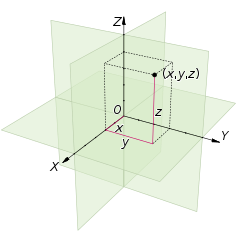
\includegraphics[]{cart.png}
\end{center}


4. Cylindrical:
A Cylindrical coordinate is a three dimensional coordinate system that specifies points position by the distance from a chosen references axis, the direction from the axis relative to a chosen reference direction and the distance from a chosen reference plane perpendicular to the axis.
Cylindrical coordinate are useful in connection with objects and phenomenum that have some rotational symmetry about the longitudinal axis , such as water flow in a straight pipe with round cross section, heat distribution in a metal cylinder , electromagnetic fields produced by an electric current in along straight wire, and so on. They are sometimes called Cylindrical polar coordinate and polar cylindrical coordinate.
\begin{center}
	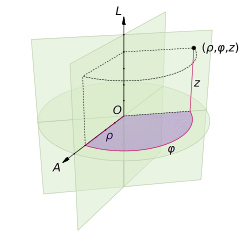
\includegraphics[]{cylindrical.png}
\end{center}


5. Spherical coordinate System:
A Spherical coordinate System is a  coordinate System  for three dimensional space where the position of a point is specified by three numbers, the radial distance of that point from a fixed origin, its polar angle measured from a fixed direction and the angle of its orthogonal projection on a reference plane that passes through the origin.
\begin{center}
	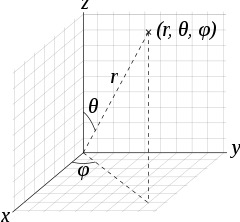
\includegraphics[width=0.47\textwidth]{spherical.png}
\end{center}


\pagebreak
\newpage

\chapter{Derivation Of Equation Of Motion in Coordinate System}
\section{Deriving continuity Equation in Cartesian Coordinate.}




\begin{center}
	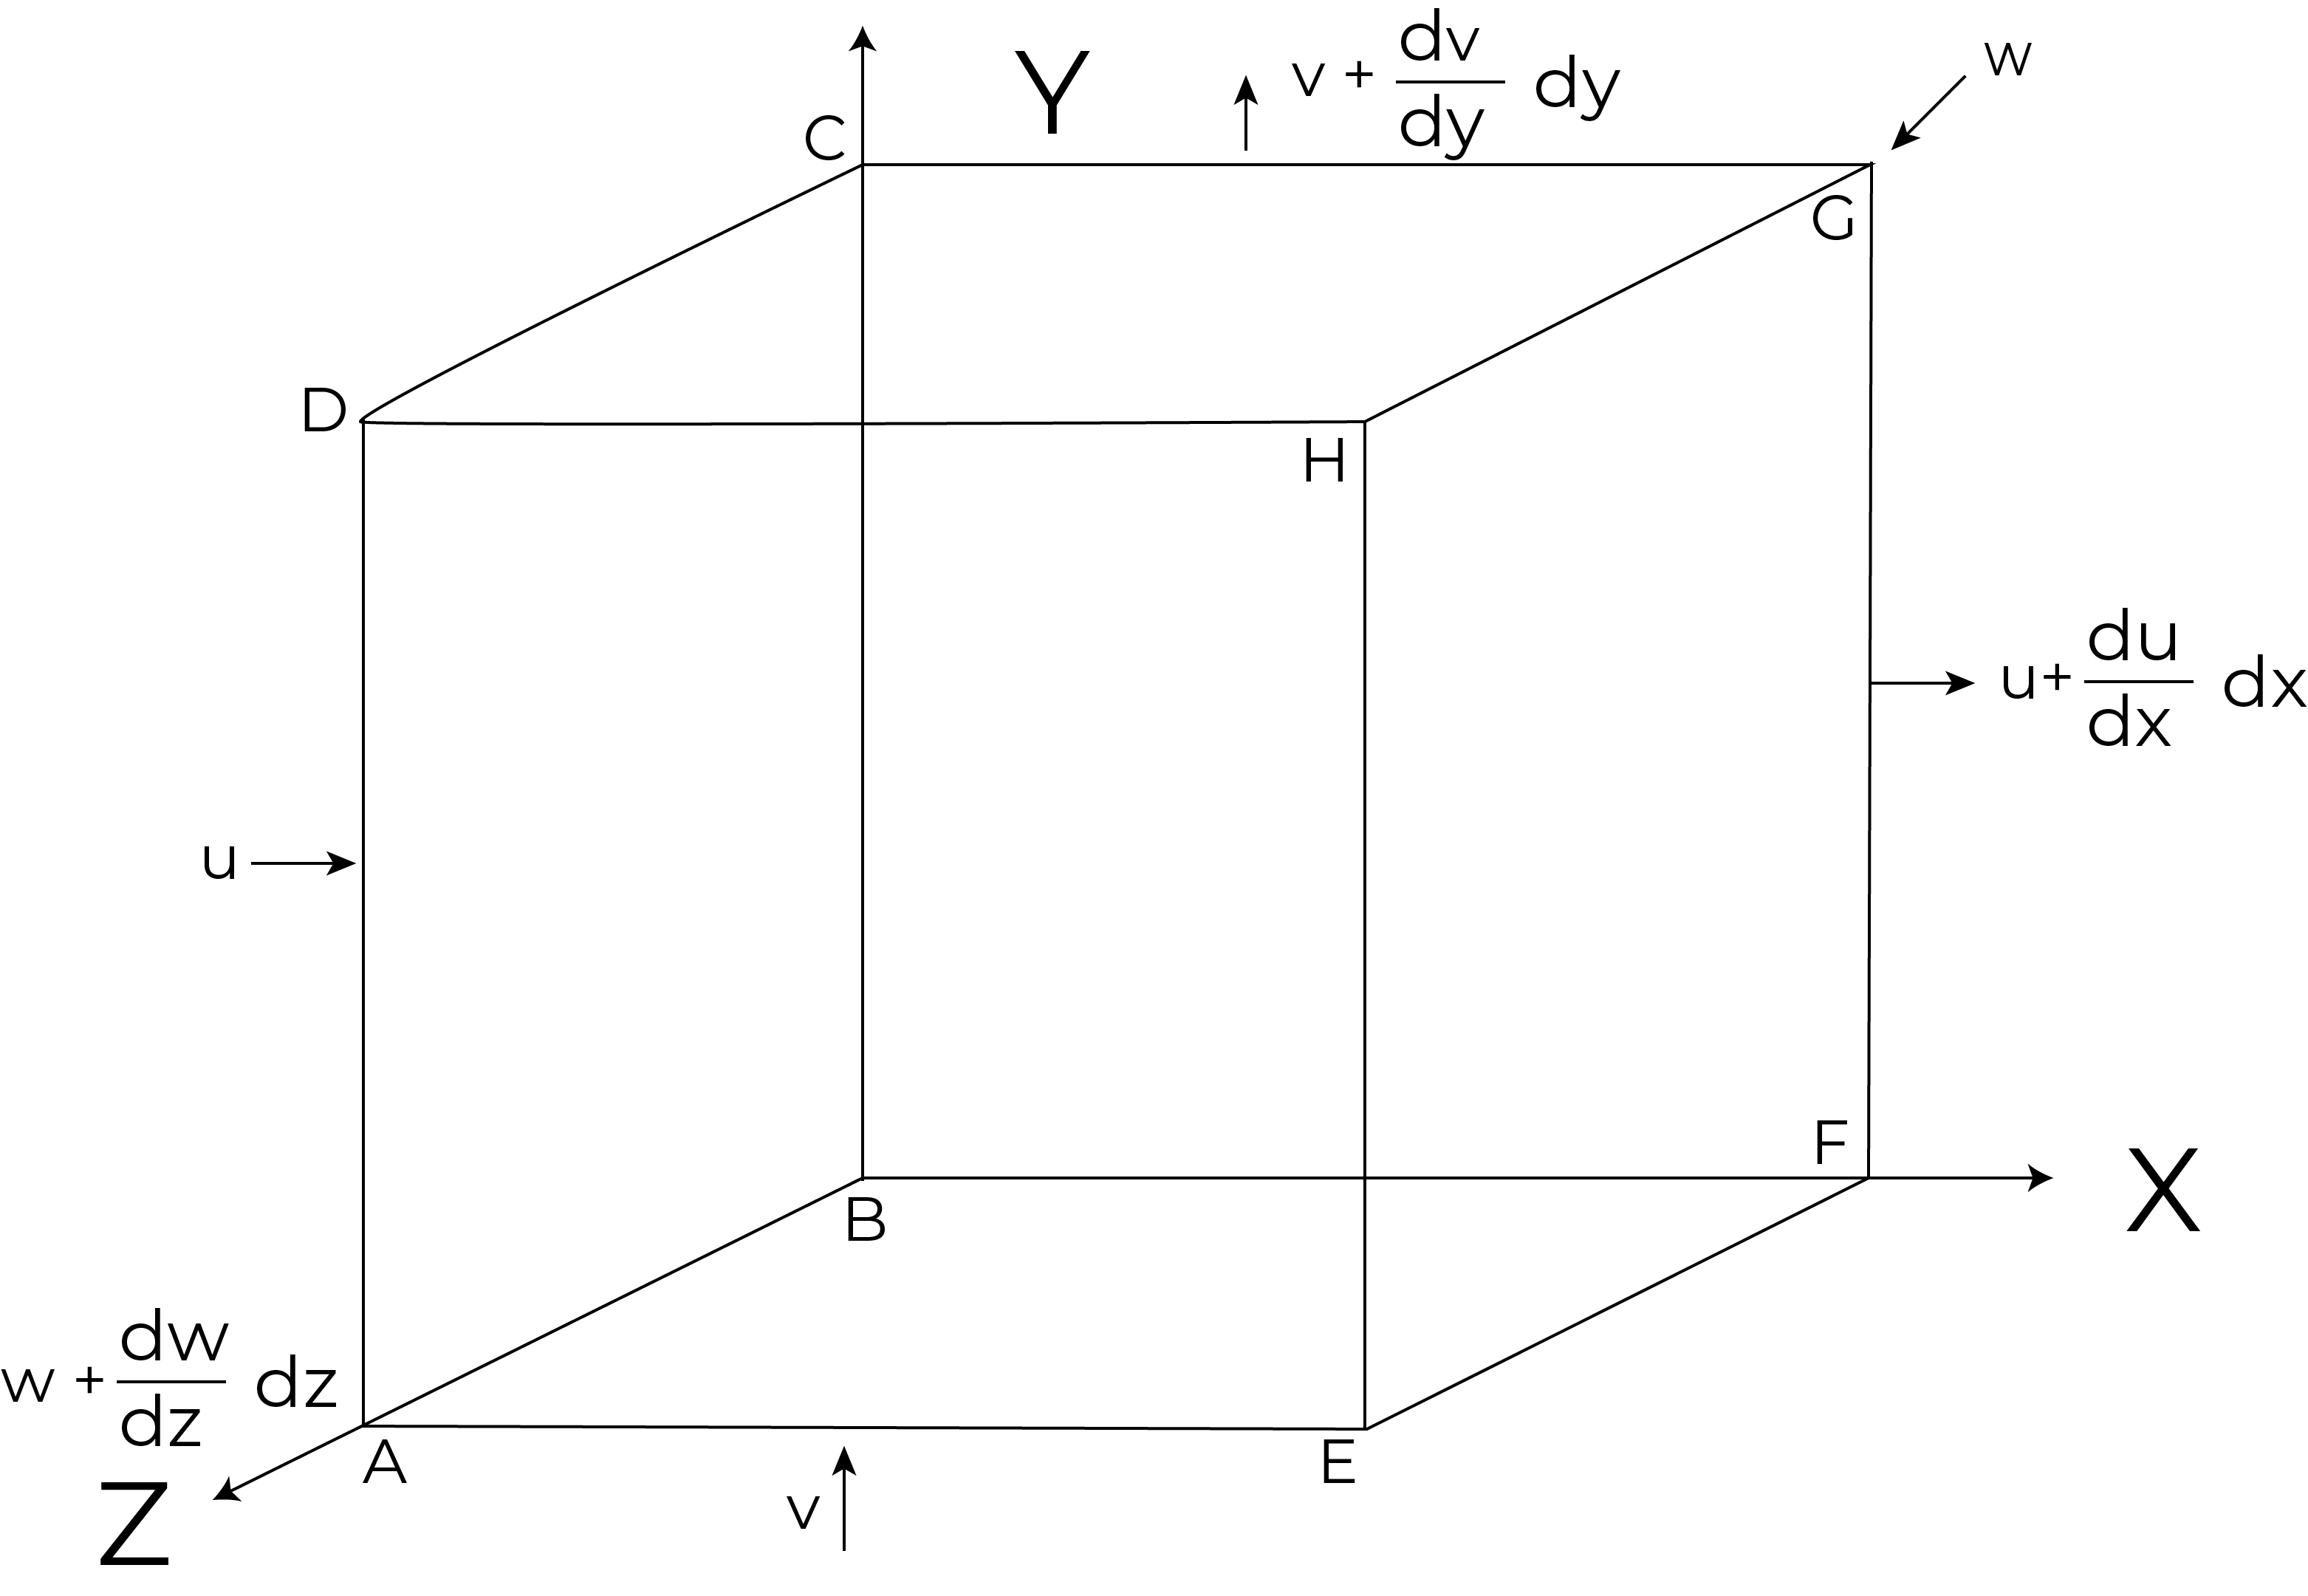
\includegraphics[width=0.57\textwidth]{cube-label0}
	
\end{center}

Mass rate entering through $ABCD$ in the diagram relating with time = $\rho u\partial y \partial z -----------(1)$

\noindent Mass rate existing through $\displaystyle EFGH = \rho(u + \frac{\partial u}{\partial x}dx)\partial y \partial z ---------(2)$\\

\noindent Net Mass rate in $X$ direction\\
equation(2) - equation (1)\\
\begin{eqnarray*}
	\rho(u + \frac{\partial u}{\partial x}dx) \partial y \partial z - \rho u \; \partial y \; \partial z &=&  \rho \frac{\partial u}{\partial x}dx \; \partial y \; \partial z\\[0.3cm]
	&=& \rho \frac{\partial u}{\partial x}du
\end{eqnarray*}

\begin{center}
	Y-Direction
\end{center}
Doing the Same Production for Y-Direction we have Net Mass rate in Y-Direction as $\displaystyle \rho \frac{\partial v}{\partial y}dv$\\
\begin{center}
	Z-Direction
\end{center}
Doing the Same Production for Z-Direction we have Net Mass rate in Z-Direction as $\displaystyle \rho \frac{\partial w}{\partial z}dw$\\

Therefore Net rate of mass leaving in the control volume = 0\\
where control volume = X-direction + Y-direction + Z-direction\\
$$
\rho \frac{\partial u}{\partial x}du + \rho \frac{\partial v}{\partial y}dv + \rho \frac{\partial w}{\partial z}dw = 0
$$
For cases of incompressible fluid $\rho = $ constant, we get the continuity equation in Cartesian coordinate.
$$
\frac{\partial u}{\partial x} + \frac{\partial v}{\partial y} + \frac{\partial w}{\partial z} = 0
$$

\subsection{Continuity Equation in Cylindrical Coordinate ($r, \phi, z$)}

\begin{center}
	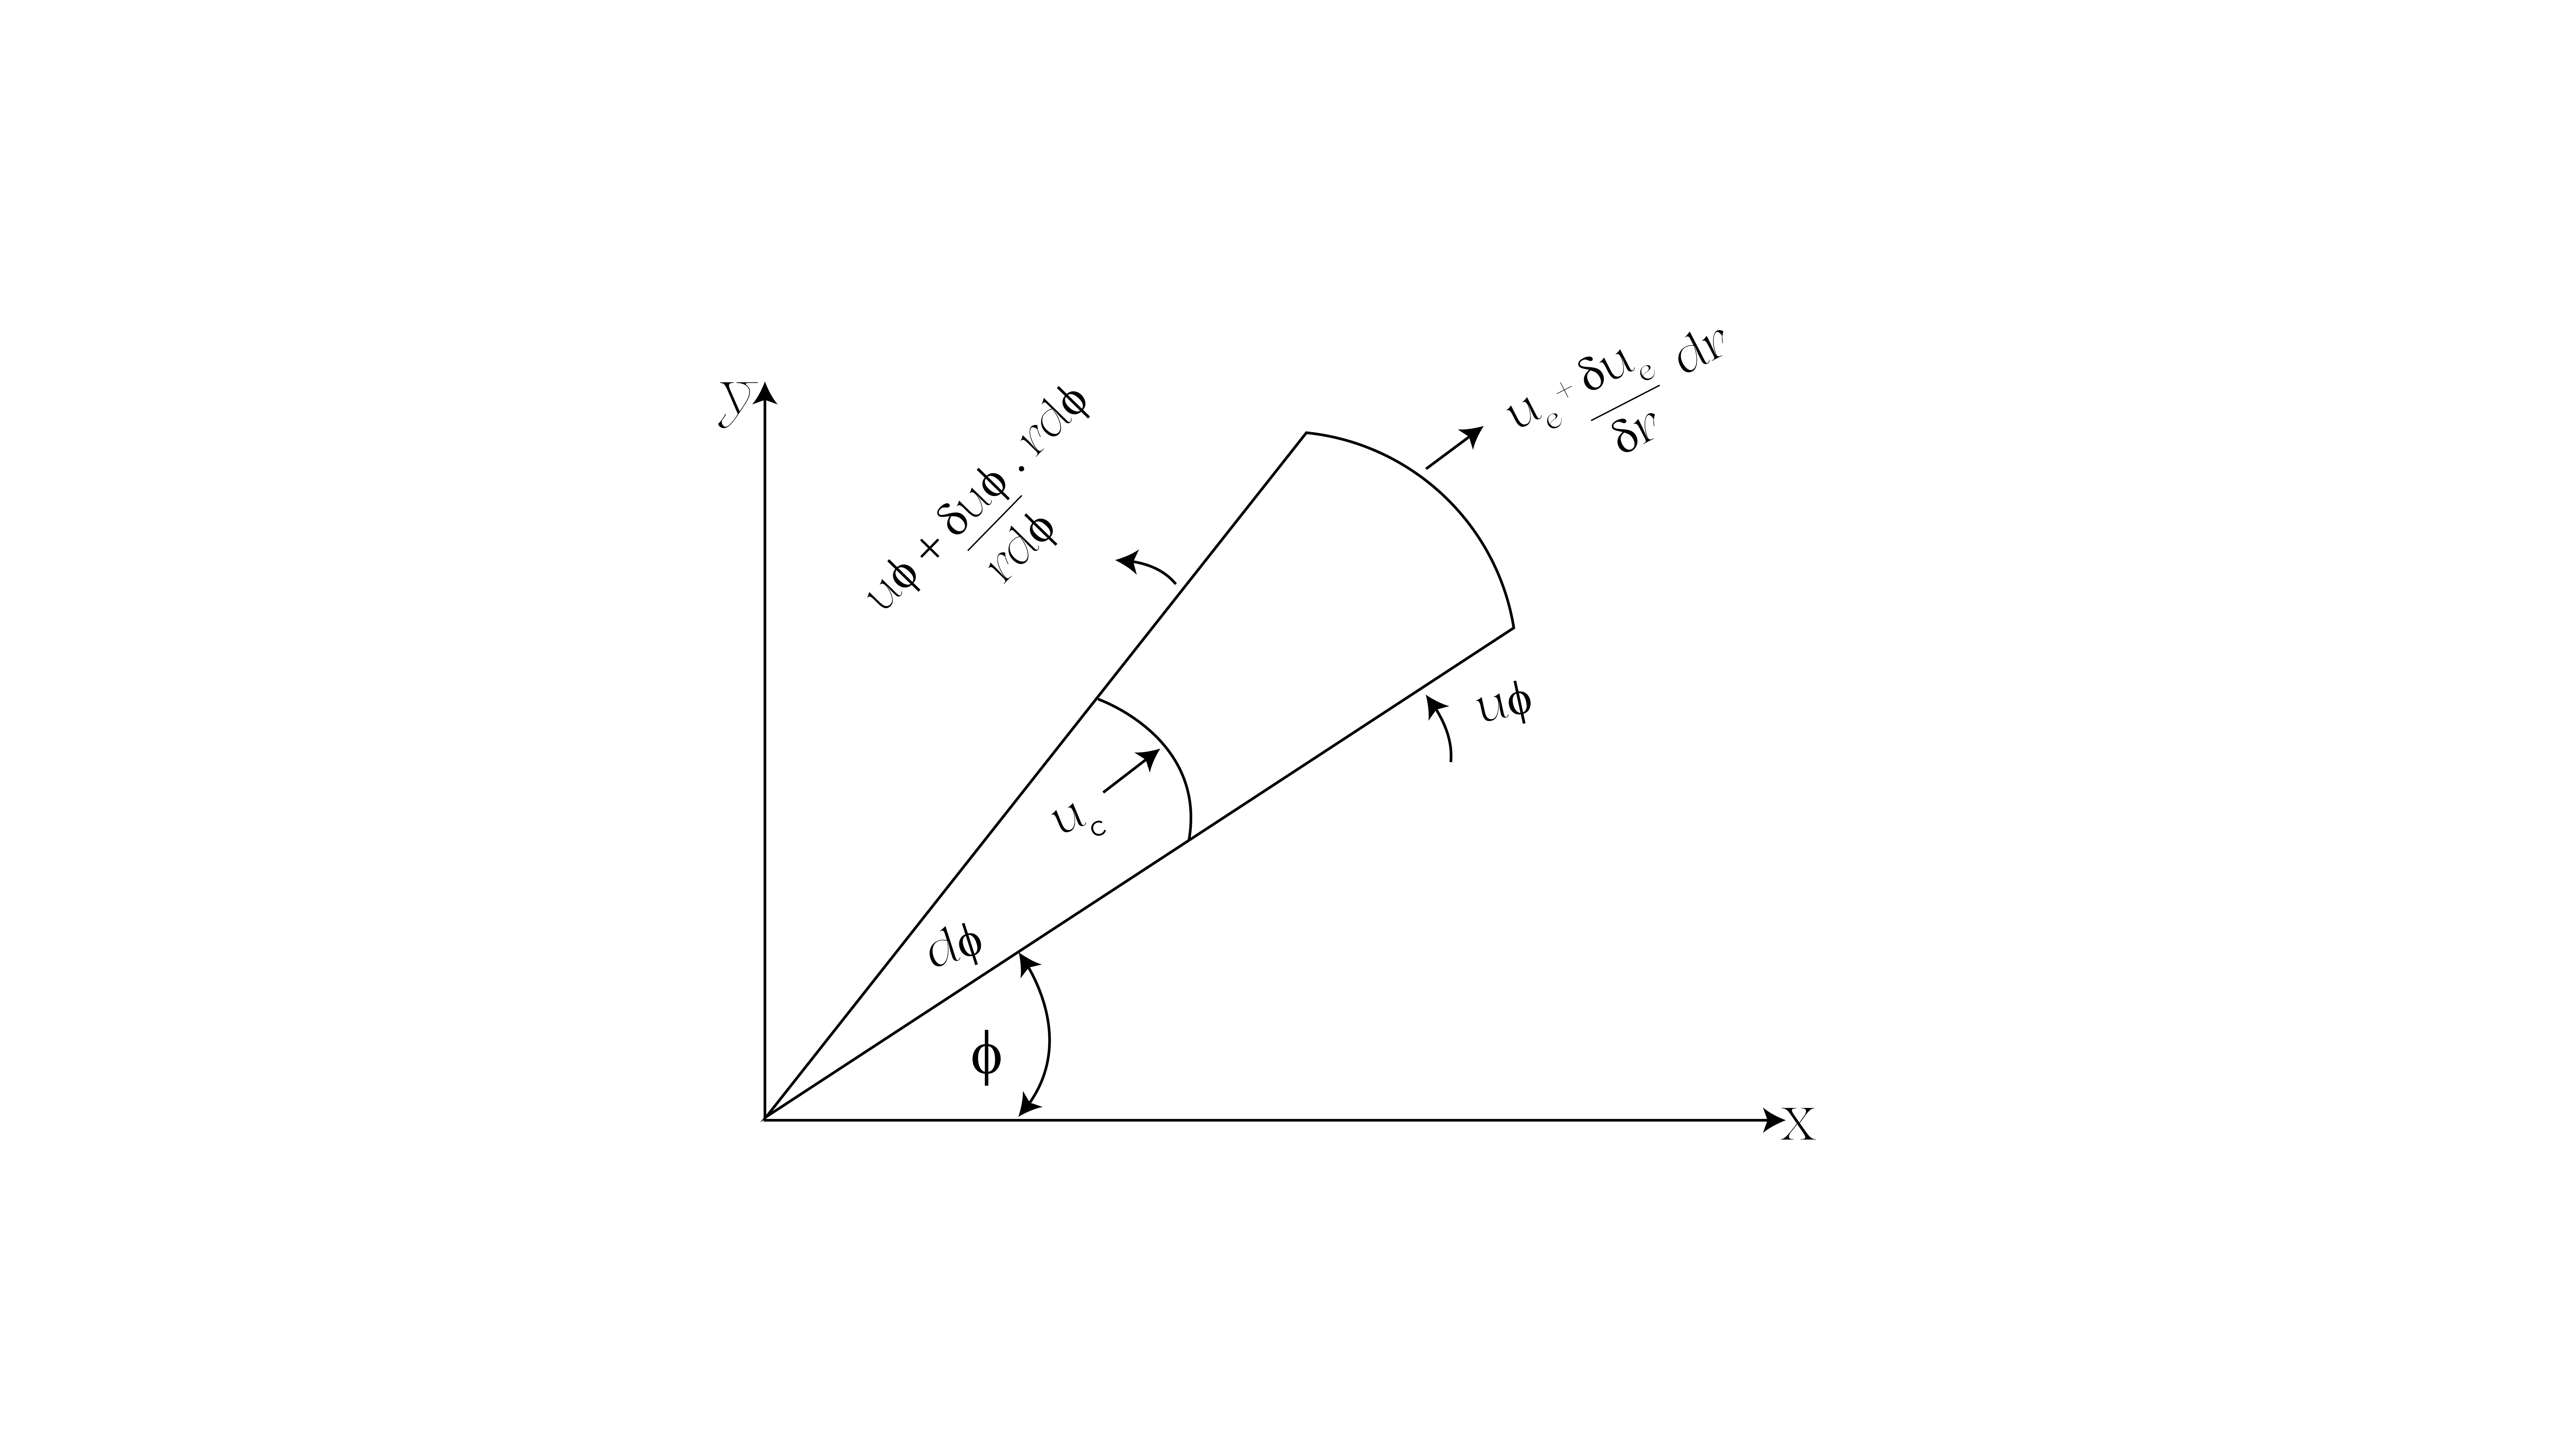
\includegraphics[width=0.97\textwidth]{bobo}
\end{center}

Mass flow rate entering radially radius (r).
$= U_c \times \rho r \; \partial\phi \;\partial z -------- (1)$\\
Mass flow rate leaving radially radius $(r+\partial r)$\\
$\displaystyle \left(u_c + \frac{\partial u_c}{\partial r}dr\right) \times \rho(r+\partial r) \partial \phi \;\partial z ---(2)$\\

$\displaystyle = u_c \;\rho(r + \partial r)\partial \phi \;\partial z + \frac{\partial u_c}{\partial r}dr \times \rho(r + \partial r)\partial\phi \;\partial z$\\

$\displaystyle = \rho \;u_c \;r\; \partial\phi\;\partial z + \rho \;u_c \;\partial r \;\partial \phi\; \partial z + \frac{\partial u_c}{\partial r}\partial r\; \partial\phi\; \partial z \; \rho\; r + \frac{\partial u_c}{\partial r}dr\;\partial r \;\partial\phi \;\rho $\\
Because $\displaystyle \frac{\partial u_c}{\partial r} dr \;\partial r \;\partial\phi \;\rho$ is small, we neglect its cause $0.1 \times 0.1 = 0.01$ is smaller\\
Net mass rate in the radial direction = eqn(2) - eqn(1)\\
$\displaystyle u_c \;\rho \;\partial r \;\partial \phi \;\partial z + \frac{\partial u_c}{\partial r} \rho\; r \;\partial\phi\; \partial r \;\partial z$\\
$$
	\text{Since }\partial \phi \partial r \partial z = \partial v
$$
$$
	= u_c\;\rho \;\partial v + \frac{\partial u_c}{\partial r}\rho\; r\;\partial v$$
$$
	= \rho\; \partial v \left(u_c + \frac{\partial u_c}{\partial r} \cdot r\right)
$$
Similarly for $\phi$ direction\\
$\displaystyle \left\{u\phi + \frac{\partial u\phi}{r\;\partial \phi}r \; \partial \phi \right\} \times \rho \; \partial r \; \partial z - u\phi\; \rho \; \partial r\; \partial z $\\[0.2cm]
$\displaystyle \left.\right. \;\; = \frac{1}{r} \frac{\partial u\phi}{\partial\phi}\; \rho \partial v $ \\[0.1cm]
Similarly for Z direction\\
$\displaystyle \left\{u_z + \frac{\partial u_z}{\partial z}\partial z\right\}\; \rho\ \partial r \; \partial \phi - u_z \; \rho\; \partial r \times r \times \partial \phi $\\[0.2cm]
$\displaystyle = u_z \rho \; \partial r \; \partial \phi + \frac{\partial u_z}{\partial z}\partial z \; \rho\;\partial r \cdot \partial \phi - u_z \rho \; \partial r \; \partial \phi $\\[0.3cm]
$\displaystyle = \frac{\partial u_z}{\partial z}\; \rho\cdot \partial r \cdot \partial z \cdot \partial \phi$\\[0.3cm]
$
 \text{ Since } \partial r \cdot \partial z \cdot \partial \phi = \partial v
 $
 $\displaystyle \frac{\partial u_z\ z}{\partial\phi}\; \rho \partial v $



$\displaystyle =\frac{\partial u_z}{\partial z} \rho  \partial v $
Therefore, Net efflux across the cylindrical control volume is zero i.e $(r + \phi + z)$ direction = 0
\begin{equation*}
	\left\lbrace \frac{u_c}{r} + \frac{\delta u_c}{\delta r} \right\rbrace + \frac{1}{r} \frac{\delta u \phi}{\delta \phi} \cdot \rho \delta v + \frac{\delta u_z}{\delta z}\ rho \delta v = 0
\end{equation*}

\begin{equation*}
	\frac{u_c}{r} + \frac{\delta u_c}{\delta r} + \frac{1}{r} \frac{\delta u \phi}{\delta \phi} + \frac{\delta u_z}{\delta z} = 0
\end{equation*}.


\subsection{DEFINITION OF THE CONTINUITY EQUATION IN SPHERICAL COORDINATION}


\begin{center}
%	\includegraphics[width=0.57\textwidth]{F:/ mama}
	
\end{center}

Selecting a spherical volume $dv$. This is given as 
\begin{equation*}
	dv=r^2sin\theta dr d\theta d\phi
\end{equation*}
Where $r,\theta,\phi$ stands for the  radius, polar and azimuthal angles respectively , the azimuthal is also reffered to as co-latitude angle.

The differential mass is 
\begin{equation*}
	dM=\rho{r^2sin\theta drd\theta d\phi}
\end{equation*}
The velocity field is represented as\newline $U=U_{er}+V_{e\theta}+W_{e\theta}$ in an eulerian reference frame mass conservation is represented by accumulation,net flow and source term in a central volume.

Accumulation is given as the time rate of change of mass\\
We therefore have
\begin{equation*}
	\frac{\partial pr^2}{\partial t}sin\theta dr d\theta d\phi
\end{equation*}
The net flow through the control volume can be divided into that corresponding to each direction.\\



\subsection{Radial Flow,(r)}
We have Min =$\rho$U $A_{in}$ the in flow are $A_{in}$ is a trapezoidal whose area is given by\newline
\begin{equation*}
	Ain=\frac{1}{2}\bigg[rsin\theta d\phi +rsin(\theta+d\theta)d\phi\bigg]rd\theta
\end{equation*}
\begin{equation*}
	\Rightarrow \sin(\theta+d\theta)=\sin\theta \cos d\theta + \cos\theta \sin d\theta \approx r^2 \sin\theta \cos\theta d\theta\\
\end{equation*}
Substituting in $A_{in}$ yields
\begin{equation*}
	A_{in}=r^2sin\theta d\theta d\phi +\frac{1}{2}r^2 cos\theta d^2\theta d\phi \approx r^2sin\theta d\theta d\phi
\end{equation*}
The out flow in radial direction is
\begin{equation*}
	M_{out}=\bigg(\rho U+\frac{\partial \rho U}{\partial r}dr\bigg)A_{out}
\end{equation*}
But ,$A_{out}$=midsegement $\times$ height\\
where mid Segment =$\frac{1}{2}\bigg[(r+dr)sin\theta d\phi +(r+dr)sin(\theta+d\theta)d\phi\bigg]$\\
Height=$(r+dr)d\theta$ \newline
\begin{equation*}
	A_{out}=r^2sin\theta d\theta d\phi +2rsin\theta dr d\theta d\phi
\end{equation*}
The net flow in the radial direction is given by
\begin{equation*}
	M_{out}-M_{in}=2\rho Ur sin\theta dr d\theta+\frac{\partial \rho U}{\partial r}r^2 sin\theta drd\theta d\phi
\end{equation*}

\subsection{Polar Flow ($\theta$)}
The inflow in the Polar direction is 
\begin{equation*}
	M_{in}=\rho VA_{in}
\end{equation*}
Where $A_{in}=rsin\theta drd\phi$
\begin{equation*}
	A_{out}=\frac{1}{2}\bigg[rsin(\theta+d\theta)d\phi +(r+dr)sin(\theta+d\theta)d\theta\bigg]dr
\end{equation*}
\begin{equation*}
	A_{out}\approx r cos\theta drd\theta d\phi +rsin\theta drd\phi
\end{equation*}
Finally, the net flow in the polar direction is 
\begin{equation*}
	M_{out}-M_{in}=\rho V_r cos \theta dr d\theta+\frac{\partial \rho V}{\partial \theta}r sin\theta dr dr\theta\phi
\end{equation*}

\subsection{ Azimuthal Flow $(\phi)$}

The inflow in the azimuthal direction is given by as\newline
$ M_{in} $= $\rho$ W $A_{in}$ \newline
 with  $A_{in}$ = r dr d $\theta$
 
 The outflow in the azimuthal direction is given by as\newline
 
\begin{equation*}
	M_{out}=(\rho W+\frac{\partial \rho W}{\partial \phi})A_{out}
\end{equation*}
and $A_{out}=rdrd\theta$\\
The net flow in polar direction is 
\begin{equation*}
	M_{out}-M_{in}=\frac{\partial \rho Wrdr}{\partial \phi}A_{out}d\theta d\phi
\end{equation*}
Now we have the continuity equation \newline
\begin{equation*}
	\frac{\partial \rho}{\partial t}dv+2\rho U\frac{d}{r}+\frac{\partial \rho u}{\partial r}+\rho Vcos\theta\frac{dv}{rsin\theta}+\frac{\partial \rho V}{\partial d\theta}\frac{dv}{r}+\frac{\partial \rho W}{\partial \phi}\frac{dv}{rsin\theta}=0
\end{equation*}

\begin{equation*}
	\frac{\partial \rho}{\partial t}+\frac{1}{2}\frac{\partial \rho r^2u}{\partial r}+\frac{1}{rsin\theta}\frac{\partial \rho vsin\theta}{\partial \theta}+\frac{1}{rsin\theta}\frac{\partial \rho W}{\partial \phi}=0
\end{equation*}


\begin{equation*}
	\frac{\partial \rho}{\partial t}+\rho \bigg(\frac{1}{r^2}\frac{\partial r^2u}{\partial r}+\frac{1}{rsin\theta}\frac{\partial vsin\theta}{\partial \theta}+\frac{1}{rsin\theta}\frac{\partial w}{\partial \phi}\bigg)=0
\end{equation*}

\newpage
\section{Derivation Of Navier stokes Equation}
The Navier stoke equation are the fundamental partial differential equation that describe the flow of incompressible fluids.

Using the rate of stress and rate of strain tensors. It can be shown that the components $F_j$ of a viscous force F on a non -rotating frame are given by \newline
\begin{equation*}
	\frac{F_i}{V}=\frac{\partial}{\partial x_j}\bigg[\eta\left(\frac{\partial u_i}{\partial x_j} +\frac{\partial u_j}{\partial x_j}+\lambda \partial_{ij}\right)\nabla .u\bigg]\quad \quad (1)
\end{equation*}
\begin{equation*}
	=\frac{\partial}{\partial x_j}\bigg[\eta(\frac{\partial u_i}{\partial x_j} +\frac{\partial u_j}{\partial x_j}-\frac{2}{3}\partial_{ij}\nabla .u\bigg]+\mu_\beta\partial_{ij}\nabla .u \quad \quad (2)
\end{equation*}


	When $\eta$ is the dynamics- viscosity. viscosity, $\lambda$ is the second viscosity,$\partial_{ij}$ is the Kroneeker delta,{$\nabla$ .u} is the divergence,$\mu$ $\beta$ is the bulk viscosity.\newline
Now for an incompressible fluid, the divergrnce $\sum\nabla .u=0$, so then the $\lambda$ terms drop out. Taking the $eta$ to be constant in spae and writing the reminder of (2) in vector form gives 
\begin{equation*}
	\frac{F_{viscous}}{V}=\eta\nabla^2 u,\quad \quad (3)
\end{equation*} 
Where $\nabla^2 u$ is the vector Laplacian.\\
There are two additional force acting on fluid parcels, namely

the pressure force.
\begin{equation*}
	\frac{F_{pressure}}{V}=-\nabla^2.P_1 \quad \quad (4)
\end{equation*}
where P is the pressure, and so called body force
\begin{equation*}
	F=\frac{F_{body}}{V}\quad \quad (5)
\end{equation*}
Adding the three forces (3),(4),(5) \& equating them to Newton's  Law of fluids yields the equation
\begin{equation*}
	\rho \frac{\partial u}{\partial t}+\rho u.\nabla u=-\nabla_p +\eta\nabla^2 u + F \quad \quad \quad (6)
\end{equation*} 
and diving through by the density $\rho$ gives
\begin{equation*}
	\frac{\partial u}{\partial t}+u.\nabla u=\frac{-\nabla p}{\rho}+\frac{\eta\nabla^2u}{\rho}+\frac{F}{\rho}
\end{equation*}
where Kinematic viscosity is $V=\frac{\eta}{\rho}$
\begin{equation}
	\frac{\partial u}{\partial t}+u.\nabla u=\frac{-\nabla p}{\rho}+V\nabla^2u+\frac{F}{\rho}\quad \quad \quad (7)
\end{equation}

The Vector equation (7) are the Navier. Stokes Equation.\\
Now consider the irrotational Navier Stokes equation in Particular co-ordinate systems\\

(1) \quad In Cartesian co-ordinate within the components of the velocity vector given by u=(u,v,w), the continuity equations.
\begin{equation*}
	\frac{\partial u}{\partial x}+\frac{\partial v}{\partial y}+\frac{\partial w}{\partial z}=0
\end{equation*}
and the Navier- Stokes are given by
\begin{equation*} 
	\rho\bigg(\frac{\partial u}{\partial t}+\mu\frac{\partial u}{\partial x}+v\frac{\partial u}{\partial y}+w\frac{\partial u}{\partial z}\bigg)=-\frac{\partial p}{\partial x}+\eta\bigg(\frac{\partial^2 u}{\partial x^2}+\frac{\partial^2 u}{\partial y^2}+\frac{\partial^2 u}{\partial z^2}\bigg)+F_x
\end{equation*}
\begin{equation*} 
	\rho\bigg(\frac{\partial v}{\partial t}+\mu\frac{\partial v}{\partial x}+v\frac{\partial v}{\partial y}+w\frac{\partial v}{\partial z}\bigg)=-\frac{\partial p}{\partial y}+\eta\bigg(\frac{\partial^2 v}{\partial x^2}+\frac{\partial^2 v}{\partial y^2}+\frac{\partial^2 v}{\partial z^2}\bigg)+F_y
\end{equation*}
\begin{equation*} 
	\rho\bigg(\frac{\partial w}{\partial t}+\mu\frac{\partial w}{\partial x}+v\frac{\partial w}{\partial y}+w\frac{\partial u}{\partial z}\bigg)=-\frac{\partial p}{\partial z}+\eta\bigg(\frac{\partial^2 w}{\partial x^2}+\frac{\partial^2 w}{\partial y^2}+\frac{\partial^2 w}{\partial z^2}\bigg)+F_z
\end{equation*}

(2) In Cylindrical Co-ordinate with the components of the velocity vector given by $U=(U_r,U_\theta,U_z)$. the continuity equation is 
\begin{equation*}
	\frac{\partial U_r}{\partial r}+\frac{U_r}{r}+\frac{1}{r}\frac{\partial u\phi}{\partial \phi}+\frac{\partial u_z}{\partial z}=0,
\end{equation*}
and the Navier- stokes equation are given by
\begin{equation*} 
	\rho\bigg(\frac{\partial u_r}{\partial t}+U_r\frac{\partial u_r}{\partial r}+\frac{U\phi}{r}\frac{\partial u_r}{\partial \phi}+U_z\frac{\partial u_r}{\partial z}-\frac{U^2\phi}{r}\bigg)
\end{equation*}
\begin{equation*} 
	=-\frac{\partial p}{\partial r}+\eta\bigg(\frac{\partial^2 u_r}{\partial r^2}+\frac{1}{r}\frac{\partial u_r}{\partial r}-\frac{U_r}{r^2}+\frac{1}{r^2}\frac{\partial^2 u_r}{\partial \phi^2}+\frac{\partial^2 U_r}{\partial z^2}-\frac{2}{r^2}\frac{\partial u_\phi}{\partial \phi}\bigg)+F_r
\end{equation*}


\begin{equation*} 
	\rho\bigg(\frac{\partial u_\phi}{\partial t}+U_r\frac{\partial u_\phi}{\partial r}+\frac{U_rU\phi}{r}\frac{U_\phi\partial u_\phi}{\partial \phi}+U_z\frac{\partial u_\phi}{\partial z}\bigg)
\end{equation*}
\begin{equation*} 
	=-\frac{1}{r}\frac{\partial p}{\partial \phi}+\eta\bigg(\frac{\partial^2 u_\phi}{\partial r^2}+\frac{1}{r}\frac{\partial u_\phi}{\partial r}-\frac{U_\phi}{r^2}+\frac{1}{r^2}\frac{\partial^2 u_\phi}{\partial \phi^2}+\frac{\partial U_\phi}{\partial z^2}-\frac{2}{r^2}\frac{\partial u_r}{\partial \phi}\bigg)+F_\phi
\end{equation*}

\begin{equation*} 
	\rho\bigg(\frac{\partial u_z}{\partial t}+U_r\frac{\partial u_z}{\partial r}+\frac{U\phi}{r}\frac{\partial u_z}{\partial \phi}+U_z\frac{\partial u_z}{\partial z}\bigg)
\end{equation*}
\begin{equation*} 
	=-\frac{\partial p}{\partial z}+\eta\bigg(\frac{\partial^2 u_z}{\partial r^2}+\frac{1}{r}\frac{\partial u_z}{\partial r}+\frac{1}{r^2}+\frac{1}{r^2}\frac{\partial^2 u_z}{\partial \phi^2}+\frac{\partial^2 u_z}{\partial z^2}\bigg)+F_z
\end{equation*}
The Spherical co-ordinate with the compound of the velocity vector gives by $U=(U_r,U_\theta,U_\phi)$ the continuity equation
\begin{equation*}
	\frac{\partial U_r}{\partial r}+\frac{2U_r}{r}+\frac{1}{r}\frac{\partial U_\theta}{\partial \theta}+\frac{U_\theta cot\theta}{r}+\frac{1}{rsin\phi}\frac{\partial U_\phi}{\partial \phi}=0
\end{equation*}
and the Navier - Stoke equation are given by 
\begin{equation*} 
	\rho\bigg(\frac{\partial u_r}{\partial t}+U_r\frac{\partial u_r}{\partial r}+\frac{U\theta}{r}\frac{\partial u_r}{\partial \theta}+\frac{U_\phi}{rsin\theta}\frac{\partial u_r}{\partial \phi}-\frac{U^2\theta}{r}-\frac{U^2\theta}{r}\bigg)
\end{equation*}
\begin{equation*} 
	=-\frac{\partial p}{\partial r}+\eta\bigg(\frac{\partial^2 u_r}{\partial r^2}+\frac{2}{r}\frac{\partial u_r}{\partial r}-\frac{2U_r}{r^2}+\frac{1}{r^2}\frac{\partial^2 u_r}{\partial \theta^2}+\frac{cot\theta}{r^2}\frac{\partial u_r}{\partial \theta}+\frac{1}{r^2sin^2\theta}\frac{\partial^2 u_r}{\partial \phi^2}-\frac{2}{r^2}\frac{\partial u_\phi}{\partial \phi}-\frac{2u_\theta}{r^2sin\theta}\frac{\partial u_\phi}{\partial\phi}\bigg)+F_r
\end{equation*}

\begin{equation*} 
	\rho\bigg(\frac{\partial u_\theta}{\partial \theta}+U_r\frac{\partial u_\theta}{\partial r}+\frac{U_rU\theta}{r}+\frac{U_\theta}{r}\frac{\partial u_\theta}{\partial \theta}+\frac{U_\phi}{rsin\theta}\frac{\partial u_\theta}{\partial \phi}-\frac{U^2\theta cot\theta}{r}\bigg)=-\frac{1}{r}\frac{\partial p}{\partial \theta}
\end{equation*}
\begin{equation*} 
	+\eta\bigg(\frac{\partial^2 u_\theta}{\partial r^2}+\frac{2}{r}\frac{\partial u_\theta}{\partial r}-\frac{U_\theta}{r^2sin^2\theta}+\frac{1}{r^2}\frac{\partial^2 u_\theta}{\partial \theta^2}+\frac{cot\theta}{r^2}\frac{\partial u_\theta}{\partial \theta}+\frac{1}{r^2sin^2\theta}\frac{\partial^2 u_\theta}{\partial \phi^2}+\frac{2}{r^2}\frac{\partial u_r}{\partial \theta}-\frac{cot\theta}{r^2sin\theta}\frac{\partial u_\phi}{\partial\phi}\bigg)+F_\theta
\end{equation*}

\begin{equation*} 
	\rho\bigg(\frac{\partial u_\phi}{\partial t}+U_r\frac{\partial u_\phi}{\partial r}+\frac{U_rU\phi}{r}+\frac{U_\phi}{r}\frac{\partial u_\phi}{\partial \theta}+\frac{U_\theta cot\theta}{r}+\frac{U_\phi}{rsin\theta}\frac{\partial u_\phi}{\partial \phi}\bigg)=-\frac{1}{rsin\theta}\frac{\partial p}{\partial \phi}
\end{equation*}
\begin{equation*} 
	+\eta\bigg(\frac{\partial^2 u_\phi}{\partial r^2}+\frac{2}{r}\frac{\partial u_\phi}{\partial r}-\frac{U_\phi}{r^2sin^2\theta}+\frac{1}{r^2}\frac{\partial^2 u_\phi}{\partial \theta^2}+\frac{cot\theta}{r^2}\frac{\partial u_\phi}{\partial \theta}+\frac{1}{r^2sin^2\theta}\frac{\partial^2 u_\phi}{\partial \phi^2}+\frac{2}{r^2sin\theta}\frac{\partial u_r}{\partial \phi}+\frac{2cot\theta}{r^2sin\theta}\frac{\partial u_\phi}{\partial\phi}\bigg)+F_\phi
\end{equation*}
The Navier-Stokes equation with no body force ($i.e F=)$ 
\begin{equation*} 
	i.e \rho\frac{\partial u}{\partial t}+\rho u.\nabla u.-\nabla p+\eta\nabla^2u.
\end{equation*}



















%%%%%%%%%%%%%%%CHAPTER FOUR%%%%%%%%%%%%%%%%%%%%
\chapter{CONVERSION OF EQUATION OF MOTION FROM CARTESIAN COORDINATE TO SPHERICAL}
\section{INTRODUCTION}
We shall be dealing with the conversion process of the continuity equation and the Navier-Stokes equation from cartesian coordinate to spherical coordinate, that is from $(X,Y,Z)$ into $(r,\theta, \phi)$.

\section{CONVERSION OF THE CONTINUITY EQUATION FROM CARTESIAN TO SPHERICAL COORDINATE}
The continuity equation in cartesian coordinate can be expressed as\sps $\dsp \frac{\partial U}{\partial x} + \frac{\partial V}{\partial y} + \frac{\partial W}{\partial z} = 0$\\

\NI Conventionally, the equation of continuity can be converted from the cartesian coordinate to the spherical coordinate by expressing $(X,Y,Z)$ as $(r, \theta, \phi)$\sps
Then\sps
$\dsp 
X = r\sin\theta\cos\phi ~~~~ r = \sqrt{x^2 + y^2 + z^2}\sps
Y = r\sin\theta\sin\phi ~~~~ r = ar\cos(\frac{z}{r})\sps
Z = r\cos \theta \qquad\quad~ \phi = \arctan(\frac{y}{z})\sps
P = r\sin \theta
$\sps 
Now the position unit vector in the spherical coordinate is given as \\
$r = Z\cos\theta + v\sin\theta$\sps
Where $v = x\cos\phi + y\sin\phi$
\begin{eqnarray}
	\frac{dr}{d\theta} &=& -Z\sin\theta + v\cos\theta\label{eq:4_1}\spn{0.5}
	%%%
	\frac{dv}{d\phi} &=& x\sin\phi + y\cos\phi\label{eq:4_2} \spn{0.5}
	%%%
	V_r &=& V_z\cos\theta + V_z\sin\theta\cos\phi + V_y\sin\theta\sin\phi \label{eq:4_3}\spn{0.5}
	%%%
	V_\theta &=& \frac{d\theta}{dt} = - \frac{dz}{dt}\sin\theta + \frac{dx}{dt}\cos\phi\cos\theta + \frac{dy}{dt}\sin\phi\cos\theta \label{eq:4_4} \spn{0.5}
	%%%
	V_\theta &=& -V_z\sin\theta + V_x\cos\phi\cos\theta + V_y\sin\phi\sin\theta \label{eq:4_5}
\end{eqnarray}
$dsp \frac{d\phi}{dt} = -\frac{dx}{dt}\sin\phi + \frac{dy}{dt}\cos\phi$\spn{0.5}
\begin{equation}
	V_\phi = -V_x\sin\phi + V_y\cos\phi \label{eq:4_6}
\end{equation}

\NI From \refn{eq:4_3} and \refn{eq:4_4} above we have
\begin{eqnarray}
	V_r &=& V_z\cos\theta + \sin\theta(V_x\cos\phi + V_y\sin\phi) \label{eq:4_7} \spn{0.1}
	%%%
	V_\theta &=& -V_{\sin\theta} + \cos\theta(V_z\cos\phi + V_y\sin\phi) \label{eq:4_8} \spn{0.1}
	%%%
	V_\phi &=& -V_x\sin\theta + V_y\cos\phi \label{eq:4_9}
\end{eqnarray}
Multiplying equation \refn{eq:4_7} and \refn{eq:4_8} through by $\cos\theta$ and $\sin\theta$ respectively, then we have
\begin{eqnarray}
	V_r\cos\theta &=& V_z\cos^2\theta + \cos\theta\sin\theta(V_x\cos\phi + V_y\sin\phi)\notag \sps
	%%%
	V_\theta\sin\theta &=& -V_z\sin^2\theta + \sin\theta\cos\theta(V_x\cos\phi + V_y\sin\phi)\notag
\end{eqnarray}
Now,
\begin{eqnarray}
	V_r\cos\theta - V_\theta\sin\theta &=& V_z\cos^2\theta + V_z\sin^2\theta \notag \sps
	%%%
	\implies V_r\cos\theta - V_\theta\sin\theta &=&V_z(\cos^2\theta + \sin^2\theta)\notag \sps
	%%%
	\implies V_z &=& V_r\cos\theta + V_\theta\sin\theta \notag
\end{eqnarray}
Multiplying equation \refn{eq:4_3} and \refn{eq:4_4} by $\sin\theta$ respectively, to have $V_r\sin\theta = V_z\cos\theta\sin\theta + \sin^2\theta(V_z\cos\phi + V_y\sin\phi)$\\
$V_\theta\cos\theta = -V_z\sin\theta\cos\theta+\sin^2\theta(V_x\cos\phi + V_y\sin\phi)$\\

\NI Now,
\begin{equation}
	V_r\sin\theta + V_theta\cos\theta = 2\sin^2\theta(V_x\cos\phi + V_y\sin\phi) \label{eq:4_10}
\end{equation}
$\dsp
\implies V_r\sin\theta + V_theta\cos\theta = V_x\cos\phi + V_y\sin\phi
$\sps
Multiplying equation \refn{eq:4_10} and \refn{eq:4_6} by $\sin\phi$ and $\cos\phi$ respectively then we have\sps
$\dsp
V_r\sin\theta\sin\phi + V_\theta\sin\phi\cos\theta = V_x\sin\theta\cos\phi + V_y\sin^2\phi \sps
%%%
V_\phi\cos\phi = -V_x\sin\theta\cos\phi + V_y\cos^2\phi \sps
%%%
= V_r\sin\theta\sin\phi + V_\theta\cos\phi\cos\theta = V_y(\sin^2\phi + \cos^2\phi)\sps
$
\begin{equation}
	\implies V_y = V_r\sin\theta\sin\phi + V_\theta\cos\phi + V_\theta\sin\phi\cos\theta \label{eq:4_11}
\end{equation}
Multiplying equation \refn{eq:4_10} and \refn{eq:4_6} by $\cos\phi$ and $\sin\phi$ respectively then we have\sps
$\dsp
V_r\sin\theta\cos\phi + V_\theta\cos\theta\cos\phi = V_x\cos^2\theta + V_y\sin\phi\cos\phi \sps
%%%
V_\phi\cos\phi = - V_x\sin^2\phi + V_y\cos\phi\sin\phi
$
\begin{equation}
	\implies V_x = V_r\sin\theta\cos\phi + V_\theta\cos\phi\sin\theta - V_\phi\sin\phi \label{eq:4_12}
\end{equation}

\NI By the general orthogonal curvilinear coordinates $(U_1,U_2,U_3)$\\
$\dsp
\nabla \cdot A = \frac{1}{h_1h_2h_3}\left[\frac{\partial}{\partial U_1}(h_1h_2A_1) + \frac{\partial}{\partial U_2}(h_1h_2A_2) + \frac{\partial}{\partial U_3}(h_1h_2A-3)\right]
$\sps
Where the scalar factors are given as\sps
$\dsp
h_1=1, h_2=r, h_3=r\sin\theta \sps
U_1=r, U_2=0, U_3=\phi \sps 
A=V = V_rx + V_\theta y+ V_\phi
$\sps
Where,\\
$\dsp
\nabla \cdot V = \frac{1}{r^2\sin\theta}\left[\frac{\partial}{\partial r}(r^2\sin\theta V_r) + \frac{\partial}{\partial \theta}(r\sin\theta V_\theta) + \frac{\partial}{\partial \phi}(rV_\phi)\right]\sps
%%%
= \frac{1}{r^2\sin\theta}\left[2r\sin\theta V_r + r^2\frac{\partial}{\partial r}\sin\theta V_r + r\cos\theta V \theta + \frac{\partial}{\partial \theta}r\sin\theta V_\theta + \frac{\partial}{\partial \phi}rV_\phi\right]\sps
%%%
=\frac{2}{r}V_r + \frac{\partial}{\partial r}V_r + \frac{\cos\theta}{r\sin\theta}V_\theta + \frac{1}{r}(2V_r + \cot\theta V_\theta)\sps
%%%
=\frac{\partial}{\partial r}V_r + \frac{1}{r}\frac{\partial}{\partial\theta}V_\theta + \frac{1}{r\sin\theta}\frac{\partial}{\partial\theta} + \frac{1}{r}(2V_r + \cot\theta V_\theta)
$\sps
Here the continuity equation in spherical coordinate is expressed as
\begin{equation*}
	\nabla \cdot V = \frac{\partial}{\partial r}V_r + \frac{1}{r}\frac{\partial}{r\partial\theta} + \frac{\partial}{\partial \phi} + \frac{1}{r}(2V_r + \cot\theta V_\theta)
\end{equation*}

\section{CONVERSION OF NAVIER-STOKES EQUATION FROM CARTESIAN TO SPHERICAL COORDINATE}
The Navier-stokes equation can be in cartesian form generally as
\begin{equation}
	\rho\left[\frac{\partial V_i}{\partial t} + V_i\frac{\partial V_j}{\partial x_i}\right] = \rho F_1 - \frac{\partial\rho}{\partial x_i} + \frac{\partial\tau_{ij}}{\partial x_j} \label{eq:4_13}.
\end{equation}
or $\dsp \rho\left[\frac{\partial V_i}{\partial t} \nabla \cdot V_jV_i\right] = \rho F_i - \nabla P + \mu\nabla^2V_i$
\begin{equation}
	\frac{\partial V_i}{\partial t} + \nabla \cdot VV_i = F_i - \frac{\nabla P}{\rho} + \upsilon\nabla^2 \Omega \label{eq:4_14}
\end{equation}
since $\upsilon = \frac{\mu}{\rho}$ By the general orthogonal coordinate $(U_1,U_2,U_3)$
\begin{equation}
	\nabla^2 = \frac{1}{h_1,h_2,h_3} \left[\frac{\partial}{\partial U_1}\left(\frac{h_1h_2}{h_1} \frac{\partial}{\partial U_2}\right) + \frac{\partial}{\partial U_2}\left(\frac{h_1h_3}{h_2}\frac{\partial}{\partial U_2}\right) + \frac{\partial}{\partial U_3}\left(\frac{h_1h_2}{h_3} \frac{\partial}{\partial U_3}\right)\right]\label{eq:4_15}
\end{equation}
Where the scalar factors are\\
$\dsp
h_1=1, h_2=r, h_3=r\sin\theta \sps
U_1=r, U_2=\theta, U_3=\phi \sps
$
\begin{equation}
	\nabla^2 = \frac{1}{r^2\sin\theta}\left[\frac{\partial}{\partial r}+ \frac{\partial}{\partial \theta}\left(\frac{r\sin\theta}{r}\frac{\partial}{\partial \theta}\right) + \frac{\partial}{\partial \pi}\left(\frac{r}{r\sin\theta}\frac{\partial}{\partial \phi}\right) \right] \label{eq:4_16}
\end{equation}
$\spn{0.7}\dsp
= \frac{1}{r^2\sin\theta}\left[2r\sin\theta\frac{\partial}{\partial r} + r^2\sin\theta \frac{\partial}{\partial r^2} + \frac{r\cos\theta}{r}\frac{\partial}{\partial \theta} + \frac{r\sin\theta}{r}\frac{\partial^2}{\partial \theta^2} + \frac{r}{r\sin\theta}\frac{\partial^2}{\partial\theta^2} \right]\sps
%%%
=\frac{2}{r}\frac{\partial}{\partial r} + \frac{\partial^2}{\partial r^2} + \frac{1}{r^2}\cos\theta\frac{\partial}{\partial\theta} +\frac{1}{r^2}\frac{\partial^2}{\partial\theta^2} + \frac{1}{r^2}\sin^2\theta\frac{\partial^2}{\partial\theta^2}
$\spn{0.6}
$\dsp
= \frac{\partial^2}{\partial r^2} + \frac{1}{r^2}\frac{\partial^2}{\partial\theta^2} + \frac{1}{r^2\sin^2\theta}\frac{\partial}{\partial\phi^2} + \frac{1}{r}\left[2\frac{\partial}{\partial r} + \frac{1}{r}\cos\theta\frac{\partial}{\partial\theta}\right]\sps
%%%
\nabla \cdot V = \frac{2}{r}V_r + \frac{\partial}{\partial r}V_r + \frac{1}{r}\cot\theta V_\theta + \frac{1}{r}\frac{\partial}{\partial\theta}V_\theta + \frac{1}{r\sin\theta}\frac{\partial}{\partial\phi}V_\theta\sps
%%%
\nabla \cdot P = \left[\frac{2}{r} + \frac{\partial}{\partial r} + \frac{1}{r}\frac{\partial}{\partial\theta} + \frac{1}{r\sin\theta}\frac{\partial}{\partial\phi}\right]\cdot P
$\sps
Substituting $\dsp \nabla^2, \nabla \cdot P, \nabla \cdot V$ into the equation \refn{eq:4_14} where $V_i$ has its velocity component as $V_r, V_\theta, V_\phi$ of spherical coordinate.\sps
\newpage
\NI In the r component\sps
$\dsp
\frac{\partial V_r}{\partial r} +V_r\frac{2V_r}{r} + V_r\frac{\partial V_r}{\partial r} + \frac{V_r}{r}\cot\theta V_\theta + \frac{V_r}{r} + \frac{\partial}{\partial\theta}V_\theta + \frac{V_r}{r\sin\theta}\frac{\partial}{\partial\phi}V_\phi\sps
$
\begin{equation}
	= g_r - \frac{1}{\rho}\left(\frac{2}{r} + \frac{\partial}{\partial r}\right)P_r + \upsilon\left[\frac{\partial^2V}{\partial r^2} + \frac{1}{r^2\sin^2\theta}\frac{\partial^2V}{\partial\phi^2} + \frac{V_r}{r}\left(\frac{2\partial}{\partial r} + \frac{1}{r}\cot\theta\frac{\partial}{\partial\theta}\right)\right] + g_r \label{eq:4_17}
\end{equation}

\NI In the $\theta$ component
\sps
$\dsp
\frac{\partial V_\theta}{\partial t} + V_\theta \frac{2V_r}{r} + V_\theta \frac{\partial V_r}{\partial r} + \frac{V_\theta}{\partial r}\cot\theta V_\theta + \frac{V_\theta}{r}\frac{\partial V_\theta}{\partial\theta} + \frac{V_\theta}{r\sin\theta}\frac{\partial}{\partial\theta}V_\phi
$
\begin{equation}
	= - \frac{1}{\rho}\left(\frac{1}{r}\cot\theta + \frac{1}{r}\frac{\partial}{\partial \theta}\right)P_\theta + \upsilon \left[\frac{\partial^2V_\theta}{\partial r^2} + \frac{1}{r^2}\frac{\partial^2V_\theta}{\partial\theta^2} + \frac{1}{r\sin\theta}\frac{\partial^2V_\theta}{\partial\phi^2} + \frac{V_\theta}{r}\left(\frac{2\partial}{\partial r} + \frac{1}{r}\cot\theta\frac{\partial}{\partial\theta}\right)\right] + g_\theta
\end{equation}

\NI In the $\phi$ component
\sps
$\dsp
\frac{\partial V_\phi}{\partial t} + V_\theta \frac{2}{r}V_r + V_\phi \frac{\partial}{\partial r} + \frac{V_\phi}{\partial r}\cot\theta V_\theta + \frac{V_\phi}{r}\frac{\partial V_\theta}{\partial\theta} + \frac{V_\phi}{r\sin\theta}\frac{\partial}{\partial\phi}V_\phi
$
\begin{equation}
	= - \frac{1}{\rho}\left(\frac{1}{r}\cot\theta + \frac{1}{r}\frac{\partial}{\partial \theta}\right)P_\theta + \upsilon \left[\frac{\partial^2V_\phi}{\partial r^2} + \frac{1}{r^2}\frac{\partial^2V_\phi}{\partial\theta^2} + \frac{1}{r\sin\theta}\frac{\partial^2V_\phi}{\partial\phi^2} + \frac{V_\phi}{r}\left(\frac{2\partial}{\partial r} + \frac{1}{r}\cot\theta\frac{\partial}{\partial\theta}\right)\right] + g_\phi
\end{equation}



%%%%%%%%%%%%%%%CHAPTER FIVE%%%%%%%%%%%%%%%%%%%%
\chapter{SUMMARY, CONCLUSION AND RECOMMENDATION}

\section{SUMMARY}
From the study of this project, FLuids were defined and explained down to its types and properties,Coordinate system were defined and also explained down to its properties and also equation of motion is explained and talked about and also  equation of motion were derived and have been converted from its cartesian to spherical coordinate and from cylindrical  to spherical coordinate in three dimensional coordinate. Considering the Navier-stokes equation and the Continuity equation which were derived from the conservation of momentum and the conservation of mass respectively.\sps

\NI These equations can be expressed as\sps
$\dsp
\frac{\Delta \rho}{\Delta t} + \rho V \cdot \overrightarrow{V} = 0 \sps
$
Which is the continuity equation and\sps
$\dsp
\rho\left(\frac{\Delta\overrightarrow{v}}{\Delta t}\right) = \rho \overrightarrow{F_i} - \nabla \overrightarrow{P} + \mu \nabla^2\overrightarrow{V}
$
respectively


\section{CONCLUSION}
The fundamental equations of motion were converted from cartesian coordinate to spherical coordinate and this was possible by applying the general orthogonal curvilinear coordinate, which has quite shown the relationship between cartesian and spherical coordinate in three dimension flow.\newline
In this study, we have employed the general orthogonal curvillinear coordinate systems to be able to convert the continuity equation and Navier-Stokes equation from cartesian coordinate to spherical coordinate.



\section{RECOMMENDATION}
 It is hereby recommended that further study should be focused on how to use the general orthogonal curvillinear coordinate to solve the conversion process of the continuity and Navier-Stokes equation from cartesian coordinate to cyclindrical coordinate, that is from $(X, Y, Z)$ into $(r,\theta,z)$.


\newpage
\chapter*{REFERENCES}
	\begin{description}
		\item Andras Alexandrou (2001), \textit{Principles of Fluid Mechanics}, Prentice Hall Upper Saddle River New Jersey.
		
		\item Bird, Robert Bryon; Stewart, Warren E,; Lightfoot, Edward N.(2007). \textit{Transport Phenomena: Wiley, Revised SEcond edition}. P. 912.ISBN 0-471-41077-2.
		
		\item Douglas, Gasiorek, Swaffield First Published in (1996) \textit{Fluid Mechanics, United Nations Educational, Kenya}.
		
		\item Egon Krause (2005), \textit{Fluid Mechanics} Springer-Verlag Berlin Heidelberg.
		
		\item Hugh D. Young, and Roger A. Freedman (2008) \textit{University Physics, Pearsons Education Inc}.
		
		\item J.N Hunt (1964). \textit{Incompressible Fluid Dynamics}.
		
		\item Reuben M. Oslon (1996) and (1961) \textit{Fluid Mechanics by International Text Book Company};. Printed in U.S.A (Second Edition).
		
	
		\item Smith, Crosbie (1998). \textit{The Science of Energy - a Cultural History of Energy Physics in Victorian Britain}. The University of Chicago Press. ISBN 978-0-226-76420-7.
		
		\item Weisstein, Eric W (1999). \textit{"Coordinate system" Math world}.
		
	\end{description}


\end{document}
